\documentclass[a4paper,12pt]{article} 

% First, we usually want to set the margins of our document. For this we use the package geometry.
\usepackage[top = 2.5cm, bottom = 2.5cm, left = 2.5cm, right = 2.5cm]{geometry} 
\usepackage[T1]{fontenc}
\usepackage[utf8]{inputenc}

% The following two packages - multirow and booktabs - are needed to create nice looking tables.
\usepackage{multirow} % Multirow is for tables with multiple rows within one cell.
\usepackage{booktabs} % For even nicer tables.

% As we usually want to include some plots (.pdf files) we need a package for that.
\usepackage{graphicx} 

% The default setting of LaTeX is to indent new paragraphs. This is useful for articles. But not really nice for homework problem sets. The following command sets the indent to 0.
\usepackage{setspace}
\setlength{\parindent}{0in}

% Package to place figures where you want them.
\usepackage{float}

% The fancyhdr package let's us create nice headers.
\usepackage{fancyhdr}

\usepackage{amsmath,amsthm,caption}
\usepackage[open]{bookmark}
\usepackage{minted}
\usepackage{paracol}


% To make our document nice we want a header and number the pages in the footer.

\pagestyle{fancy} % With this command we can customize the header style.

\fancyhf{} % This makes sure we do not have other information in our header or footer.

\lhead{\footnotesize Operating System (H): Assignment 4}% \lhead puts text in the top left corner. \footnotesize sets our font to a smaller size.

%\rhead works just like \lhead (you can also use \chead)
\rhead{\footnotesize Mengxuan Wu} %<---- Fill in your lastnames.

% Similar commands work for the footer (\lfoot, \cfoot and \rfoot).
% We want to put our page number in the center.
\cfoot{\footnotesize \thepage} 

\begin{document}

\thispagestyle{empty} % This command disables the header on the first page. 

\begin{tabular}{p{15.5cm}}
{\large \bf Operating System (H)} \\
Southern University of Science and Technology \\ Mengxuan Wu \\ 12212006 \\
\hline
\\
\end{tabular}

\vspace*{0.3cm} %add some vertical space in between the line and our title.

\begin{center}
	{\Large \bf Assignment 4}
	\vspace{2mm}

	{\bf Mengxuan Wu}
		
\end{center}  

\vspace{0.4cm}

\section*{Question 1}

During address translation, the CPU hardware is responsible for
\begin{enumerate}
	\item Remember the base and bound values for currently running process.
	\item Perform the translation of virtual address to physical address.
	\item Raise an exception if the process tries to access an illegal address.
	\item Support instructions to let the operating system change the base and bound registers, but not user mode programs.
\end{enumerate}

The operating system is responsible for
\begin{itemize}
	\item Allocating and de-allocating memory for processes.
	\item Remember the base and bound registers for each process, and load them into the CPU when the process is scheduled.
	\item Handling the exception raised by the CPU when a process tries to access an illegal address.
\end{itemize}

In general, the OS tells the CPU what the base and bound registers should be, and what handler should be called when an exception is raised. The CPU performs the actual address translation with the given base and bound registers, and raises an exception if the address is illegal.

\section*{Question 2}

\begin{paracol}{2}
\begin{center}
	\textbf{Segmentation}
\end{center}
\switchcolumn
\begin{center}
	\textbf{Paging}
\end{center}
\end{paracol}

\textbf{Size of chunks}

\begin{paracol}{2}
Size of chunks is variable. OS can allocate memory of different sizes to different chunks.
\switchcolumn
Size of chunks is fixed (e.g., page size).
\end{paracol}

\textbf{Management of free space}

\begin{paracol}{2}
Free space is tracked by the OS. When a process requests memory, the OS finds a free chunk of the appropriate size (always contiguous) and gives it to the process.
\switchcolumn
Free space is tracked by the OS. When a process requests memory, the OS finds one or more free pages (could be non-contiguous) and gives them to the process.
\end{paracol}

\textbf{Context switch overhead}
\begin{paracol}{2}
The OS needs to load the segmentation table for the new process and change corresponding registers. 
\switchcolumn
The OS needs to change the base address register of page table for the new process and flush the TLB.
\end{paracol}

\textbf{Fragmentation}
\begin{paracol}{2}
Segmentation can cause external fragmentation. If the OS cannot find a contiguous chunk of memory, it cannot allocate memory to the process.
\switchcolumn
Paging solves the problem of external fragmentation. The OS can allocate non-contiguous pages to a process.
\end{paracol}

\textbf{Status bits}
\begin{paracol}{2}
Segmentation can have status bits to indicate growth direction, read/write/execute permissions.
\switchcolumn
Paging can have status bits to indicate read/write/execute permissions, valid/invalid pages (valid bit), dirty/clean pages (dirty bit), present/absent pages (present bit), accessed/not accessed pages (accessed bit).
\end{paracol}

\section*{Question 3}

Three levels of page tables are required.

Since the page size is 8KB, the offset is 13 bits. For 46-bit virtual addresses, we need $46 - 13 = 33$ bits for the page number. Since each page table entry is 4 bytes, we can fit $8 \text{KB} / 4 \text{B} = 2^{11}$ entries in each page table. Therefore, we need $33 / 11 = 3$ levels of page tables.

The format of the virtual address is as follows:
\begin{table}[H]
	\centering
	\begin{tabular}{|c|c|c|c|}
		\hline
		11 bits (Level 1) & 11 bits (Level 2) & 11 bits (Level 3) & 13 bits (Offset) \\
		\hline
	\end{tabular}
\end{table}

\section*{Question 4}

\subsection*{(a)}

The page size is $2^{12} = 4 \text{KB}$, since the offset is 12 bits.

Then $32 - 12 = 20$ bits are left for the page number. The maximum page table size is $2^{20} \times 4 \text{B} = 4 \text{MB}$.

\subsection*{(b)}

For \texttt{0xC302C302}, the first-level page number is \texttt{0x30C} (10 bits), and the offset is \texttt{0x302} (12 bits).

For \texttt{0xEC6666AB}, the second-level page number is \texttt{0x266} (10 bits), and the offset is \texttt{0x6AB} (12 bits).

\section*{Question 5}

\begin{figure}[H]
	\centering
	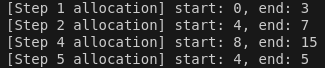
\includegraphics[width=0.8\linewidth]{figure/buddy.png}
\end{figure}

For the first allocation, the buddy system allocates the initial 4 frames to the process. For the second allocation, the buddy system allocates 4 frames, following the first 4 frames. Then the second 4 frames are de-allocated. Now the whole memory is segmented into:
\begin{itemize}
	\item 4 frames allocated to the process.
	\item 4 frames free.
	\item 8 frames free.
	\item 16 frames free.
	\item 32 frames free.
\end{itemize}

Thus, when requesting 8 frames, the buddy system will allocate the 8 frames starting from the 8th frame. And the memory is segmented into:
\begin{itemize}
	\item 4 frames allocated to the process.
	\item 4 frames free.
	\item 8 frames allocated to the process.
	\item 16 frames free.
	\item 32 frames free.
\end{itemize}

Then, 2 frames are allocated. The buddy system splits the first 4 free frames into 2 frames and 2 frames. The memory is segmented into:
\begin{itemize}
	\item 4 frames allocated to the process.
	\item 2 frames allocated to the process.
	\item 2 frames free.
	\item 8 frames allocated to the process.
	\item 16 frames free.
	\item 32 frames free.
\end{itemize}
\end{document}